\documentclass{article}
\usepackage{xeCJK}
\usepackage{amsmath}
\usepackage{amssymb}
\usepackage{mathrsfs}
\usepackage{xcolor}
\usepackage{bm}
\usepackage{hyperref}
\usepackage{graphicx}
\usepackage{subcaption}
\usepackage{float}
\usepackage{multicol}
\usepackage{pdfpages}
\usepackage{csquotes}
\usepackage[ruled,linesnumbered]{algorithm2e}
\usepackage[numbers, sort&compress]{natbib}

\bibliographystyle{plain}
\setlength{\parindent}{2em}
\usepackage{geometry}
\geometry{a4paper, left=2.54cm, right=2.54cm, top=3.18cm, bottom=3.18cm}

% set line spacing
% \renewcommand{\baselinestretch}{1.5}

% define reference format
\hypersetup{
    colorlinks=true,
    linkcolor=blue,
    urlcolor=blue,
    citecolor=blue,
    linkbordercolor=white
}

\title{\textbf{Phase Frustration-Induced Spatial Lattice Symmetry in the Vicsek-Kuramoto-Sakaguchi Model}}
\author{Yichen Lu}

\begin{document}

\maketitle

\tableofcontents

% \newpage
\section{The Model}

Particles are described by position $\mathbf{r}_i=\left( x_i, y_i \right)$ and phase angle $\theta_i$, evolving as:
\begin{subequations} 
    \label{eq:totalDynamicsMeanField}
    \begin{align}
        \dot{\mathbf{r}}_i&=v\mathbf{p}\left( \theta _i \right)\;\label{eq:dotR},
        \\
        \dot{\theta}_i&=\frac{K}{\left| A_i \right|}\sum_{j\in A_i}{\left[ \sin \left( \theta _j-\theta _i+\alpha \right) -\sin \alpha \right]}\;\label{eq:dotTheta},
    \end{align}
\end{subequations}
where $A_i\left( t \right) =\left\{ j: \left| \mathbf{r}_i\left( t \right) -\mathbf{r}_j\left( t \right) \right|\leqslant d_0 \right\}$ is the set of neighbors within coupling radius $d_0$, $K \left(\geqslant 0\right)$ is coupling strength, and $\alpha$ is frustration.
The term $-\sin\alpha$ ensures synchronization ($\theta_j = \theta_i$) remains an equilibrium \cite{10.1143/PTP.79.1069}.
This model generalizes alignments \cite{PhysRevLett.119.058002,PhysRevResearch.1.023026,Escaff2020,PhysRevLett.127.238001,PhysRevLett.133.258302}, anti-alignments \cite{PhysRevE.109.024602,PhysRevE.110.024603}, and chimera states \cite{PhysRevE.98.032219,PhysRevE.102.022604}. It reduces to normal Vicsek–Kuramoto for $\alpha=0$ and anti-aligning interactions for $\alpha=\pi$.

\newpage
\section{Simulation Results}

\begin{figure}[H]
    \centering
    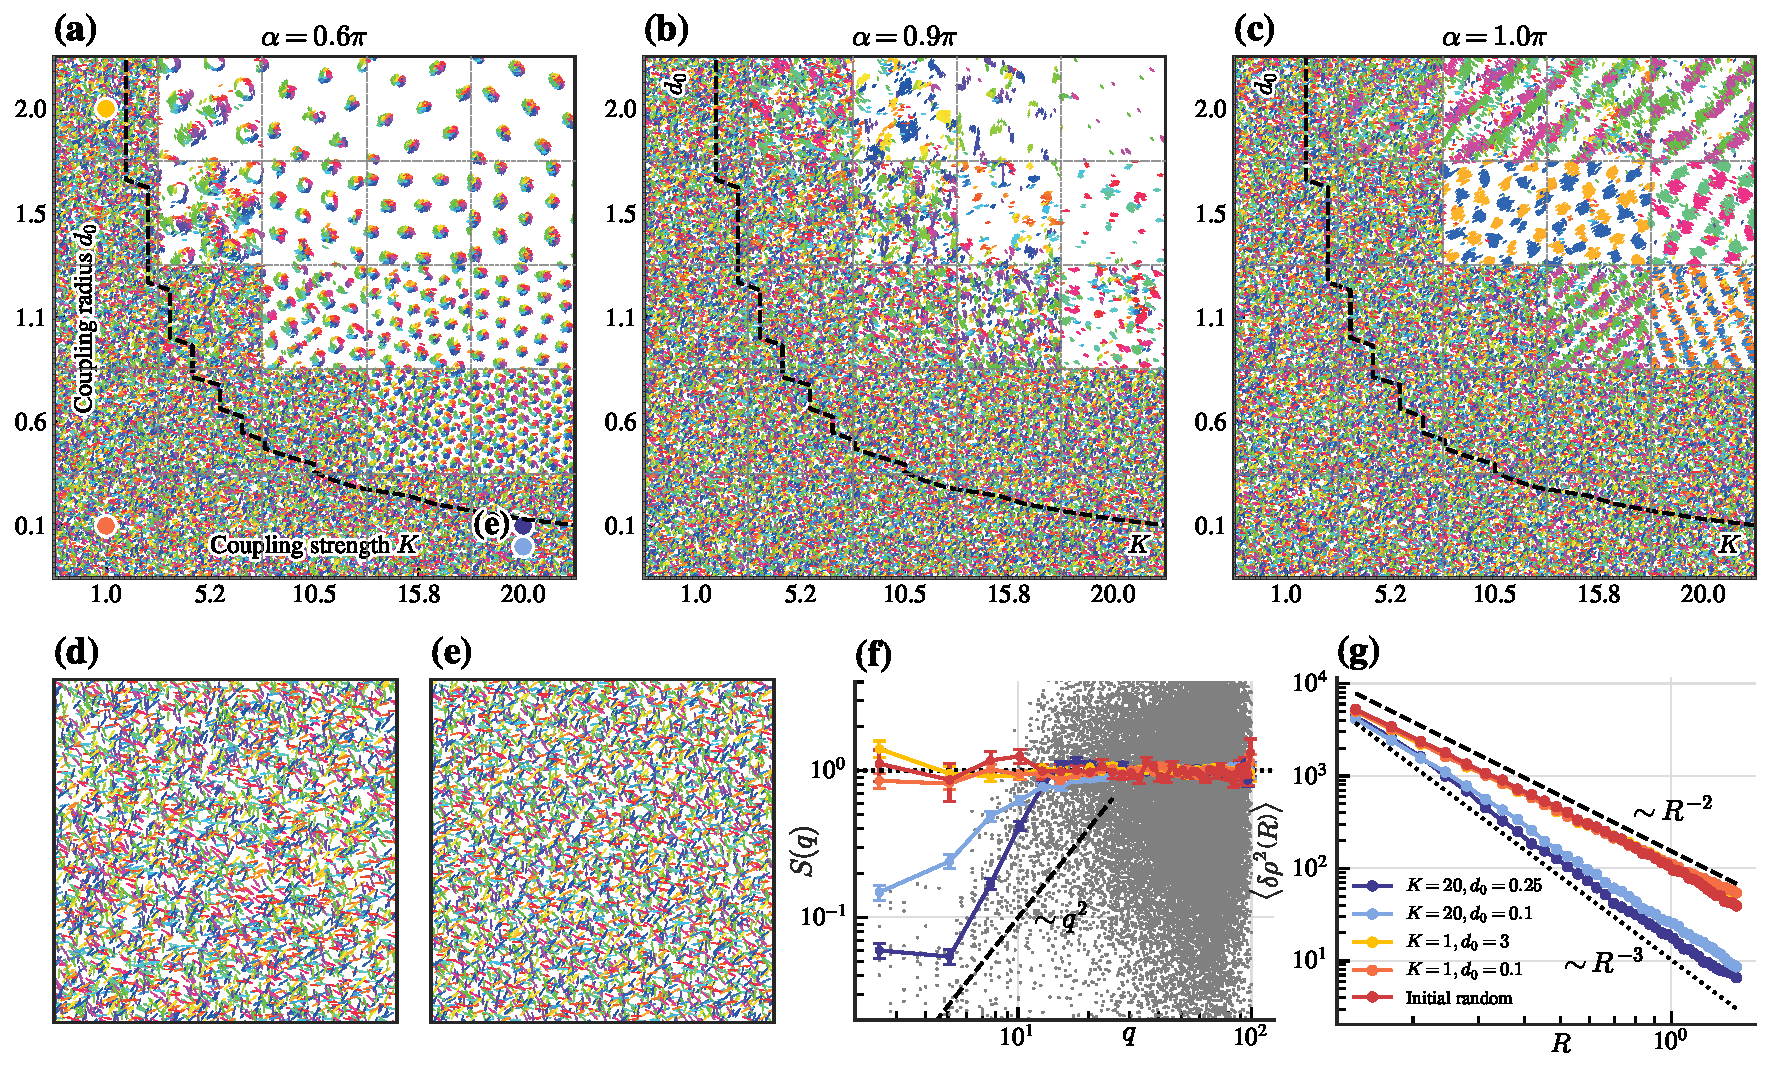
\includegraphics[width=\textwidth]{./figs/phaseDiagramAndHyperuniformity.pdf}
    \caption{
        \label{fig:phaseDiagramAndHyperuniformity}
        (a)-(c) Snapshots of $(K, d_0)$ phase diagram under different frustration $\alpha$ for $L=7, N=2000$ and $v=3$. The boundaries between dominant and recessive lattice states, are indicated with black dashed lines.
        (d), (e) Snapshots comparing random uniform initial conditions (d) and the resulting hyperuniform final state (e) for $K=20, d_0=0.25, \alpha=0.6\pi$ and $N=5000$ (large population for better showcase).
        Hyperuniformity of the recessive lattice states is characterized by the structure factor $S(q)$ in (f) and the density variance $\langle \delta \rho ^2\left( R \right) \rangle $ in (g). 
        Black dashed lines indicate the scaling behaviors $S(q)\sim q^{-2}$ and $\langle \delta \rho ^2\left( R \right) \rangle\sim R^{-2,-3}$, respectively.
        In (f), gray dots represent the sample of $S(\mathbf{q}_{\mathbf{n}})$ for periodic boundary conditions allowed wavevectors $\mathbf{q}_{\mathbf{n}}=(2\pi n_1/L,2\pi n_2/L)$ with $\mathbf{n}\in \left( \mathbb{Z} ^* \right) ^2$ at $K=20, d_0=0.25$, and the point-fold curves with error bars show the binned average and standard deviation of their respective $S(\mathbf{q}_{\mathbf{n}})$.
        Solid dots and text label in (a) mark the location in $(K, d_0)$ phase diagram corresponding to the parameters analyzed in (e)-(g).
    }
\end{figure}

\begin{figure}[H]
    \centering
    \subcaptionbox{
        Structure factor $S(\mathbf{q})$
    }[0.49\linewidth]{
        \includegraphics[width=\linewidth]{figs/Sq_vs_q_hyperuniformity_vary_K.pdf}
    }
    \hfill
    \subcaptionbox{
        Density fluctuation variance $\left< \delta \rho ^2 \right>$
    }[0.49\linewidth]{
        \includegraphics[width=\linewidth]{figs/density_fluctuation_variance_vary_K.pdf}
    }
    \caption{
        (a) Structure factor $S(\mathbf{q})$ for varying coupling strength $K$ for $\alpha=0.6\pi, d_0=0.1$. (b) Density fluctuation variance $\left< \delta \rho ^2 \right>$ as a function of mean density $\left< \rho \right>$ for different $K$ values.
    }
\end{figure}

\begin{figure}[H]
    \centering
    \subcaptionbox{
        Structure factor $S(\mathbf{q})$
    }[0.49\linewidth]{
        \includegraphics[width=\linewidth]{figs/Sq_vs_q_hyperuniformity_vary_K_d0_0.25.png}
    }
    \hfill
    \subcaptionbox{
        Density fluctuation variance $\left< \delta \rho ^2 \right>$
    }[0.49\linewidth]{
        \includegraphics[width=\linewidth]{figs/density_fluctuation_variance_vary_K_d0_0.25.png}
    }
    \caption{
        (a) Structure factor $S(\mathbf{q})$ for varying coupling strength $K$ for $\alpha=0.6\pi, d_0=0.25$. (b) Density fluctuation variance $\left< \delta \rho ^2 \right>$ as a function of mean density $\left< \rho \right>$ for different $K$ values.
    }
\end{figure}

\newpage
\begin{figure}[H]
    \centering
    \includegraphics[width=0.7\textwidth]{./figs/forward.png}
    \caption{
        Forward snapshots.
    }
\end{figure}

\begin{figure}[H]
    \centering
    \includegraphics[width=0.7\textwidth]{./figs/backward.png}
    \caption{
        Backward snapshots.
    }
\end{figure}

\begin{figure}[H]
    \centering
    \includegraphics[width=0.5\textwidth]{./figs/K_vs_slope.pdf}
    \caption{
        The slope of $S(q)$ in the small-$q$ regime as a function of coupling strength $K$ at fixed frustration $\alpha=0.6\pi$.
    }
\end{figure}

\begin{figure}[H]
    \centering
    \subcaptionbox{
        Structure factor $S(\mathbf{q})$
    }[0.49\linewidth]{
        \includegraphics[width=\linewidth]{figs/Sq_vs_q_hyperuniformity_vary_d0.pdf}
    }
    \hfill
    \subcaptionbox{
        Density fluctuation variance $\left< \delta \rho ^2 \right>$
    }[0.49\linewidth]{
        \includegraphics[width=\linewidth]{figs/density_fluctuation_variance_vary_d0.pdf}
    }
    \caption{
        (a) Structure factor $S(\mathbf{q})$ for varying coupling radius $d_0$ at fixed frustration $\alpha=0.6\pi$. (b) Density fluctuation variance $\left< \delta \rho ^2 \right>$ as a function of mean density $\left< \rho \right>$ for different $K$ values.
    }
\end{figure}

\bibliography{ref}

\end{document}